\chapter{PROPOSED HEURISTIC ALGORITHM} \label{ch_distOracle}
%Chapter 4
%%%%%%%%%%%%%%%%%%%%%%%%%%%%%%%%%%%%%%%%%%%%%%%%%%%%%%%%%%%%%%%%%%%%%%%%%%%%%%%%%%%%%%%%%%%%%%%%%%%%%%%%%%%%%%%%%%%%%%
\section{Overview}
In this chapter, we propose a new heuristic approximation algorithm for the Steiner tree algorithm with a new running time complexity for this algorithm, this running time is totally depend on the order of the edges present in the graph, new running time will be order of $O(|S||V|log|V|)$ for the sparse graph and $O(|S||V|log|V| + |E||S|)$ approx $O(|S||V|^2)$ for the other graphs, where $|S|$ is the number of terminal nodes and $|V|$ is the number of vertex nodes in the graph $G$. Even we are getting the same running time for the graphs which have edges of order $|E|$ > $|V|log|V|$ but we are reducing the steps of the algorithms. This running time, we are getting with the help of a shortest path finding algorithm between the vertices, for that we are using all-pairs shortest-paths algorithm. In this algorithm a graph $G = (V,E)$, is given as a input.

 The $\emph{all pairs shortest path}$ problem on $G$ is to compute the minimum distance between the vertices of graph $G$. In this proposal, we are presenting, how we are reducing the running time complexity of our algorithm $algo1$ as given in the previous chapter with the help of some other algorithm. So for that we are using all-pairs shortest-path algorithm for finding the shortest path between the pairs of vertices. In this part we are presenting how, we will use the goodness of all-pairs shortest path algorithm, for finding the Steiner tree in a given graph $G$ by using the heuristic algorithm $algo1$ presented in the previous chapter, the running time complexity for that algorithm is $O(|S||V|^2)$, which is approximate to $|V|^3$ if all vertices are terminals.

 Here we are presenting the improved version of that algorithm $algo1$, with the help of the Dijkstra's algorithm, we are using this algorithm for finding the shortest path between the pairs of vertices. As we know that the time bound for the Dijkstra's is $O(|V|log|V| + |E|)$, if we implement min-priority queue with the help of fibonacci heap. In algorithm $algo1$ most of the running time taken by the step 1, so we have to think about that step only, how to reduce the running time for this step and rest of steps are taking some what linear or $O(|V|^2)$ running time, so overall running time for that algorithm was $O(|S||V|^2)$. If we use the all-pairs shortest-path algorithm for finding the minimum distance between vertices, they we come up with a new running time complexity of $O(|S||V|log|V|)$ for the graph the graph which have $|E|$ $<$ $|V|log|V|$ and $O(|S||V|log|V| + |E||S|)$ for the other graphs, this is done by running the Dijkstra's algorithm from each vertices as a source i.e., $|S|$ times. 

\subsection{Modification in The All-pairs Shortest-Path Algorithm}
Here modification for finding the shortest path between the pairs of vertex, in this algorithm we run the Dijkstra's algorithm for every vertices present in the graph for to find the minimum distance between source and destination. But in the modified algorithm instead of running Dijkstra's algorithm for each and every pairs vertices for finding the shortest path between then, as for our heuristic algorithm it is required to find the shortest distance between the terminals only, so if we run the Dijkstra's algorithm from each and every terminal taking as a source of the algorithm. For finding the shortest path between every pair of terminals, we have to run the Dijkstra's algorithm from every terminals i.e., $|S|$ times. Our Dijkstra's algorithm will take $O(|S||V|log|V| + |E||S|)$ times for finding the shortest path between all-pairs of vertices in $G$, if we find the shortest path between the all pairs of terminals by running the Dijkstra's algorithm from every terminal as a source and rest of the vertices as the destination for the Dijkstra's algorithm. Then we have to run Dijkstra's algorithm almost $O(|S|)$ times to find the shortest path between every pairs of terminals, and total running time will be $O(|S||V|log|V|)$ for the graphs which have number of edges $O(|E|)$ $<$ $|V|log|V|$ and $O(|S||V|logV + |E||S|)$ for the other graphs, where $O(|V|log|V| + |E|)$ is the running time for the Dijkstra's algorithm ~\cite{dijktra}, and we are running the Dijkstra's algorithms $|S|$ times, as total number of terminals in a given graph $G$ are $|S|$. So worst case running time for finding the shortest path between each and every pairs of terminals will be $O(|S||V|log|V| + |E||S|)$, this is achieved by running the Dijkstra's algorithm from every terminals.

We are just running the Dijkstra's algorithm from every terminals of the graph $G$, and finding the shortest path between the every pair of the terminals, so we can say that the running time complexity for this algorithm will be $O(|S||V|log|V|)$ and $O(|S||V|log|V| + |E||S|)$, which we can say that, this is better running time than the previous algorithm's running time for algorithm $algo1$ which was $O(|S||V|^2)$ and we are skipping some of the steps of algorithm $algo1$, but now we have a algorithm $algo2$ with running time $O(|S||V|log|V|)$ for the graphs which have edges of $|E|$ $<$ $|V|log|V|$ and $O(|S||V|log|V| + |E||S|)$ for the other graphs for finding the minimum distance between the terminals, with the help this we construct a subgraph between having the minimum distance between the terminals present in the graph $G$, as we constructed in the step 3rd of heuristic algorithm $algo1$. 

\begin{lemma} \label{hitsel}
In a graph $G$ = $(V,E)$ such that $S \subseteq V$, where $S$ is the terminals of the graph $G$, then we can stated that the running  time of the algorithm will be $O(|S||V|log|V|)$ $\leq$ $O(|V|^2log|V|)$. 
\end{lemma}

Modified algorithm is use to find the minimum distance between pairs of vertices in a graph. If we run dijkstra's algorithm from every pair of the terminal and find the shortest-path between other terminals. The Dijkstra's algorithm discover the path by using the optimal edges in shortest path, while pruning the other unnecessary edges that are not useful in shortest path.\\

\subsection{Approximation Algorithm for Steiner Tree}
Here we are presenting the description of the modified approximation algorithm for the Steiner tree, with a better running time. We start with a heuristic algorithm and explanation of that by using graphs. 

\textbf{Heuristic Algorithm :- }\\
Heuristic Algorithm for construct a Steiner tree from a graph. Given a connected graph $G$, and edges weight or cost is the minimum distance $d$ between two vertices $v_i$ and $v_j$ if there is a edge. We are given some require vertices S, S is the subset of vertices S$\subseteq$V. A path is a sequence of vertices, $(v_1,v_2,v_3 \dots, v_n)$, a path from a vertex $v_1$ to $v_n$ going through the vertices $(v_2,v_3 \dots, v_{n-1})$~\cite{karger}. A symbol ($u$ $\leadsto$ $v$) is used for path representation from $u$ to $v$ (if there exits a edge between ($u$,$v$)). A simple path is a path in which all the vertices are distinct. Sum of the path is the sum of weights of all the edges which are used in the path. A Shortest path is the path between the vertices $v_1$ to $v_n$ whose path sum is minimum among all the possible paths from $v_1$ to $v_n$. A loop is a path, $(v_1,v_2,v_3 \dots, v_n)$, such that $v_1$ = $v_n$. Here we are presenting algorithm $algo2$ for finding the Steiner tree in given graph $G$ as a input.\\ A Steiner tree is a tree that cover all the required vertices with the minimum distance. This algorithm $algo2$ is the 3 steps algorithm for finding the Steiner tree. The Steiner tree produced by algorithm suggested heuristic algorithm is not necessarily minimal. However, it will be shown that the total distance $D_H$ will not be very far from the $D_{MIN}$, $D_{MIN}$ is the total distance of the minimum Steiner tree. We have shown approximation ratio 2$\Big(1-\frac{1}{|S|}\Big)$ in $Algo1$, where $|S|$ is the number of terminals in the graph~\cite{markowsky}.


\begin{tabular}{|ll|} 
 \hline
 \multicolumn{ 2}{|l|}{\problemfontbold{Algorithm $algo2$:- }} \\
 \emph{INPUT} & \begin{minipage}[t]{0.9\columnwidth}
 A undirected connected graph $G$ = $(V,E)$ with edge distance or cost $d$ between the vertices $v_i$ and $v_j$, and a subset of nodes $S \subseteq V$, $S$ is called required vertex.
 \end{minipage} \\
 \emph{OUTPUT} & \begin{minipage}[t]{0.8\columnwidth}
 A Steiner Tree $T_s$ = $(V_s,E_s)$ of G and S.\\
 \end{minipage}\\
 \emph{Step 1.} & \begin{minipage}[t]{0.9\columnwidth}
  Given a graph $G$ and required vertices($S$) as input, we construct a subgraph $G$ $_s$, from that graph $G$. This subgraph having the shortest path between each and every pairs of terminals. This construction will be done by running Dijkstra's algorithm considering each terminal as a source. \\
 \end{minipage}
 \\
  \emph{Step 2.} & \begin{minipage}[t]{0.9\columnwidth}
 From that subgraph $G_s$ find a minimum spanning tree, by applying one of the minimum spanning tree algorithm like prim's algorithm.(If more that minimum spanning trees are present in the subgraph, pick arbitrary one, as all are minimum spanning tree so their weight will be same).\\
 \end{minipage}
 \\
 \emph{Step 3.} & \begin{minipage}[t]{0.9\columnwidth}
 From the minimum spanning tree, delete all unnecessary edges which are not connecting the required vertices(S). Do deletion till there is no leaves as non-terminal. Final tree after this, so called as the Steiner tree(No Steiner nodes as leaves).\\
 \end{minipage}
 \\
 \hline
 \end{tabular}
 \\

In this algorithm running time taken by each Step, Step 1 running time $O(|S||V|log|V| +|E||S|)$ this running time depend on the order of $O(E)$ in the graph, if order of edges $|E|$ < $|V|log|V|$ than overall running time will be $O(|S||V|log|V|)$ which is better than the previous algorithm $algo1$ but other graph which don't have edges of order $|E|$ < $|V|log|V|$ for that running time will be $O(|S||V|log|V| +|E||S|)$ totally depends on the number of the edges present in the graph. As we are applying the Dijkstra's algorithm on every terminals of the graph and total number of terminals are $|S|$, so we have to run Dijkstra's algorithm $|S|$ times to get the shortest distance for each and every pairs terminals of the graph, we know running time for Dijkstra's algorithm is $O(|V|log|V| +|E|)$, which we are applying $|S|$ times, so total running time of our step 1 will be $O(|S||V|log|V| +|E||S|)$ but for the graph which have edges $|E|$ < $|V|log|V|$ like sparse graph for that graphs running time will be $O(|S||V|log|V|)$. Step 2 could be done in $O(|V|^2)$ time and Step 3 can be done in $O(|V|)$ time, as our previous algorithm $algo1$ is taking. So running time complexity for our algorithm $algo2$ will be $O(|S||V|log|V|)$ for the sparse graph and $O(|S||V|log|V| + |E||S|)$ for the other graphs. Even we are getting the running time approximately same for some of the graphs which have $|E|$ > $|V|log|V|$, but we are reducing the steps in our heuristic algorithm. Here, we are explaining each and every step of our new heuristic algorithm by taking the same graph as a example.\\

Example:
\begin{figure}[H]
\begin{center}
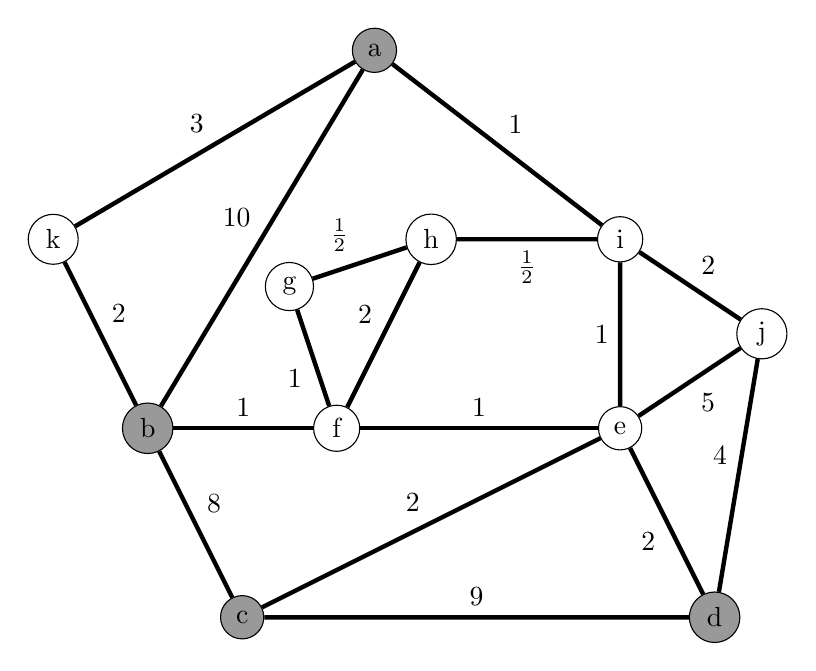
\begin{tikzpicture}[scale=1.2, auto, node distance=2cm,
   node_style/.style={circle,draw=black},
   edge_style/.style={draw=black, ultra thick}]

    \node[node_style, fill=black!40] (v1) at (0.4,4) {a};
    \node[node_style, fill=black!40] (v2) at (-2, 0) {b};
    \node[node_style] (v11) at (-3, 2) {k};
    \node[node_style, fill=black!40] (v3) at (-1,-2)  {c};
    \node[node_style, fill=black!40] (v4) at (4,-2)  {d};

    \node[node_style] (v5) at (3,0) {e};
    \node[node_style] (v6) at (0,0)  {f};
    \node[node_style] (v7) at (-0.5,1.5) {g};
    \node[node_style] (v8) at (1,2) {h};
    \node[node_style] (v9) at (3,2)  {i};
    \node[node_style] (v10) at (4.5,1) {j};
    % \node[node_style] (v10) at (2,-2) {l};
    % \node[node_style,fill=black!40] (v11) at (4,-3) {c};
    % \node[node_style,fill=black!40] (v12) at (3,2)  {e};
    \draw[edge_style]  (v2) edge node{1} (v6);
    \draw[edge_style]  (v2) edge node{10} (v1);
    \draw[edge_style]  (v2) edge node{8} (v3);
    \draw[edge_style]  (v1) edge node{1} (v9);
    \draw[edge_style]  (v9) edge node{$\frac{1}{2}$} (v8);
    \draw[edge_style]  (v7) edge node{$\frac{1}{2}$} (v8);
    \draw[edge_style]  (v6) edge node{1} (v7);
    \draw[edge_style]  (v6) edge node{1} (v5);
    \draw[edge_style]  (v4) edge node{2} (v5);
    \draw[edge_style]  (v3) edge node{9} (v4);
    % \draw[edge_style]  (v3) edge node{8} (v2);
    \draw[edge_style]  (v3) edge node{2} (v5);
    \draw[edge_style]  (v5) edge node{1} (v9);
    \draw[edge_style]  (v9) edge node{2} (v10);
    \draw[edge_style]  (v10) edge node{5} (v5);
    \draw[edge_style]  (v4) edge node{4} (v10);
    \draw[edge_style]  (v6) edge node{2} (v8);
    \draw[edge_style]  (v11) edge node{3} (v1);
    \draw[edge_style]  (v11) edge node{2} (v2);
    
    
    
    \end{tikzpicture}
    % \caption{\small \sl Torricelli point X \label{fig:sccEx} }
    \caption{Connected weighted Graph G, with Steiner vertices(hollow), and 4 terminal vertices(dark)}
    \end{center}
    
    % \caption{\small \sl  }
    \end{figure}

 \begin{figure}[H]
\centering
\begin{subfigure}{.5\textwidth}
  \centering
       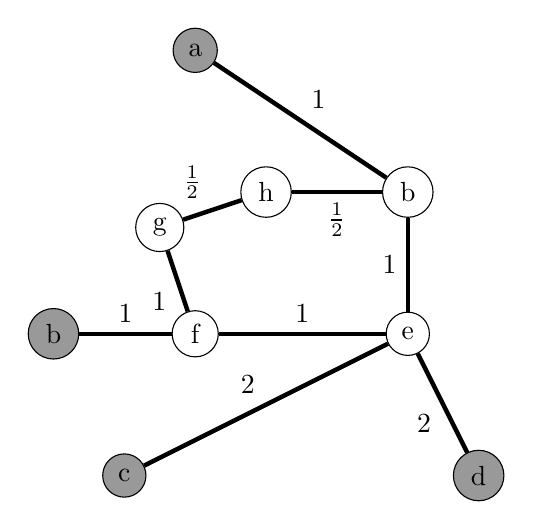
\begin{tikzpicture}[scale=0.9, auto, node distance=2cm,
   node_style/.style={circle,draw=black},
   edge_style/.style={draw=black, ultra thick}]

    \node[node_style, fill=black!40] (v1) at (0,4) {a};
    \node[node_style, fill=black!40] (v2) at (-2, 0) {b};
    \node[node_style, fill=black!40] (v3) at (-1,-2)  {c};
    \node[node_style, fill=black!40] (v4) at (4,-2)  {d};

    \node[node_style] (v5) at (3,0) {e};
    \node[node_style] (v6) at (0,0)  {f};
    \node[node_style] (v7) at (-0.5,1.5) {g};
    \node[node_style] (v8) at (1,2) {h};
    \node[node_style] (v9) at (3,2)  {b};
    \draw[edge_style]  (v2) edge node{1} (v6);
    % \draw[edge_style]  (v2) edge node{10} (v1);
    % \draw[edge_style]  (v2) edge node{8} (v3);
    \draw[edge_style]  (v1) edge node{1} (v9);
    \draw[edge_style]  (v9) edge node{$\frac{1}{2}$} (v8);
    \draw[edge_style]  (v7) edge node{$\frac{1}{2}$} (v8);
    \draw[edge_style]  (v6) edge node{1} (v7);
    \draw[edge_style]  (v6) edge node{1} (v5);
    \draw[edge_style]  (v4) edge node{2} (v5);
    % \draw[edge_style]  (v3) edge node{9} (v4);
    % \draw[edge_style]  (v3) edge node{8} (v2);
    \draw[edge_style]  (v3) edge node{2} (v5);
    \draw[edge_style]  (v5) edge node{1} (v9);
    \end{tikzpicture}
  
  % \includegraphics[width=.4\linewidth]{image1}
  \caption{A sub-graph $G_s$ of G }
  % \label{fig:sub1}
\end{subfigure}%
\begin{subfigure}{.5\textwidth}
  \centering
  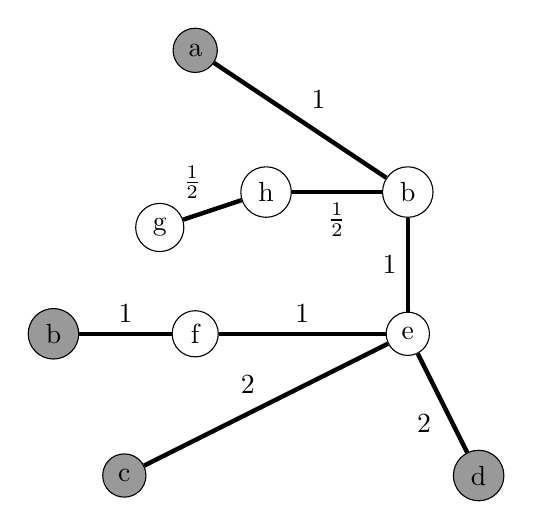
\begin{tikzpicture}[scale=0.9, auto, node distance=2cm,
   node_style/.style={circle,draw=black},
   edge_style/.style={draw=black, ultra thick}]

    \node[node_style, fill=black!40] (v1) at (0,4) {a};
    \node[node_style, fill=black!40] (v2) at (-2, 0) {b};
    \node[node_style, fill=black!40] (v3) at (-1,-2)  {c};
    \node[node_style, fill=black!40] (v4) at (4,-2)  {d};

    \node[node_style] (v5) at (3,0) {e};
    \node[node_style] (v6) at (0,0)  {f};
    \node[node_style] (v7) at (-0.5,1.5) {g};
    \node[node_style] (v8) at (1,2) {h};
    \node[node_style] (v9) at (3,2)  {b};
    \draw[edge_style]  (v2) edge node{1} (v6);
    % \draw[edge_style]  (v2) edge node{10} (v1);
    % \draw[edge_style]  (v2) edge node{8} (v3);
    \draw[edge_style]  (v1) edge node{1} (v9);
    \draw[edge_style]  (v9) edge node{$\frac{1}{2}$} (v8);
    \draw[edge_style]  (v7) edge node{$\frac{1}{2}$} (v8);
    % \draw[edge_style]  (v6) edge node{1} (v7);
    \draw[edge_style]  (v6) edge node{1} (v5);
    \draw[edge_style]  (v4) edge node{2} (v5);
    % \draw[edge_style]  (v3) edge node{9} (v4);
    % \draw[edge_style]  (v3) edge node{8} (v2);
    \draw[edge_style]  (v3) edge node{2} (v5);
    \draw[edge_style]  (v5) edge node{1} (v9);
    
    \end{tikzpicture}
  % \includegraphics[width=.4\linewidth]{image1}
  \caption{Minimum spanning tree from subgraph graph $G_s$}
  % \label{fig:sub2}
\end{subfigure}


%%%%%%%%%%%%%%%%%%%%%%%%%%%%%%%%%%%%%%%%%%%%%%%%%%%%%%%%%%%%%%%%%%%%%%%%%%%%%%%%%

% \begin{figure}
\begin{center}
    % \caption{\small \sl Torricelli point X \label{fig:sccEx} }
    \end{center}
\end{figure}
% \label{fig:sccEx}



\begin{figure}[H]
\begin{center}
\begin{subfigure}{.5\textwidth}

  \centering
  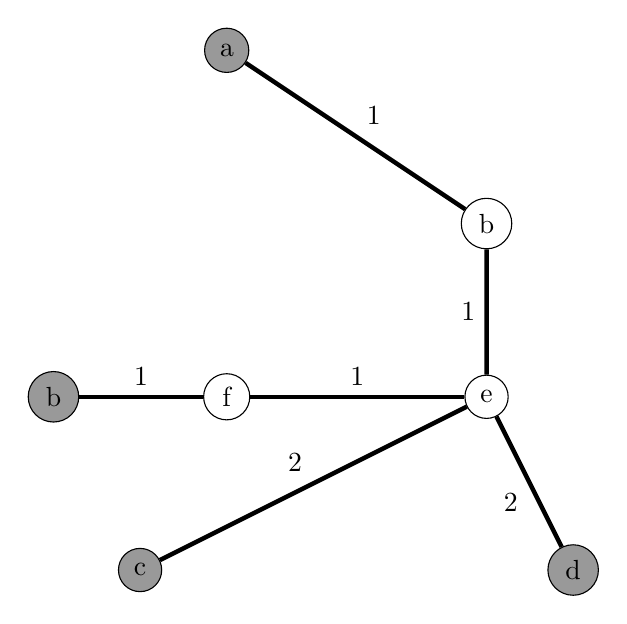
\begin{tikzpicture}[scale=1.1, auto, node distance=2cm,
   node_style/.style={circle,draw=black},
   edge_style/.style={draw=black, ultra thick}]

    \node[node_style, fill=black!40] (v1) at (0,4) {a};
    \node[node_style, fill=black!40] (v2) at (-2, 0) {b};
    \node[node_style, fill=black!40] (v3) at (-1,-2)  {c};
    \node[node_style, fill=black!40] (v4) at (4,-2)  {d};

    \node[node_style] (v5) at (3,0) {e};
    \node[node_style] (v6) at (0,0)  {f};
    \node[node_style] (v9) at (3,2)  {b};
    \draw[edge_style]  (v2) edge node{1} (v6);
    \draw[edge_style]  (v1) edge node{1} (v9);
    \draw[edge_style]  (v6) edge node{1} (v5);
    \draw[edge_style]  (v4) edge node{2} (v5);
    \draw[edge_style]  (v3) edge node{2} (v5);
    \draw[edge_style]  (v5) edge node{1} (v9);
    \end{tikzpicture}

  
  % \includegraphics[width=.4\linewidth]{image1}
  \caption{Steiner tree for Graph $G$}
  % \label{fig:sub2}
\end{subfigure}
\end{center}
\caption{All the steps of our algorithm are cover by above graph, final Steiner tree is shown figure 4.2(e).}
% \label{fig:test}
\end{figure}
In figure 4.1 we are given a graph $G$ with 4 terminals vertices shown as dark. we are required to find the minimal cover of these terminals only. From that graph $G$ we construct a subgraph $G_s$ as shown in figure 4.2(a). After constructing subgraph $G_s$ as shown in figure 4.2(a), we apply step 2nd of our algorithm i.e., minimum spanning tree algorithm on that subgraph.\\ Minimum spanning tree of subgraph $G_s$ is shown in figure 4.2(b), on that minimum spanning tree we apply 3rd step of our algorithm and we come up a minimal cover of the terminals, this is called as the Steiner tree of graph $G$.


\section{Input Dataset Description}

The input instances are taken from DIMACS website $(www://steinlib.zib/testset.php)$, which contain several dataset for the Steiner tree problem.
instance dataset that, we used in our implementation.\\

\textbf{1. P4E Dataset :-} P4E dataset instances are random generated complete graphs with euclidian weights.\\
In these instance $DC$ column classifies the difficulty of the instance ~\cite{koch}.\\
When we run both the algorithm $algo1$  and $algo2$ on the dataset description in the table 4.1, $algo1$ is given heuristic and $algo2$ is proposed algorithm.
In figure 4.3, as we observe that the running time for our algorithm $algo2$ is almost better than the algorithm $algo1$ in all the cases.\\
As we observe in all cases more is the $Opt$ more is the difference in the running time.\\ 

\begin{table}[ht]
% \caption{My caption}
\label{my-label}
\begin{center}
\begin{tabular}{|l|l|l|l|l|l|}
\hline
Name & $|V|$      & $|E|$      & $|S|$      & DC         & Opt       \\ \hline
P455    &  100       &  4950      &    5   &  Ps         &  1138  \\ \hline
P456    &  100       &  4950      &    5   &  Ps         &  1228  \\ \hline
P457    &  100       &  4950      &    5   &  Ps         &  1609  \\ \hline
P458    &  100       &  4950      &    5   &  Ps         &  1868  \\ \hline
P459    &  100       &  4950      &    5   &  Ps         &  2345  \\ \hline
P460    &  100       &  4950      &    5   &  Ps         &  2959  \\ \hline
P461    &  100       &  4950      &    5   &  Ps         &  4474  \\ \hline
P463    &  200       &  19900     &    20  &  Ps         &  1510  \\ \hline
P465    &  200       &  19900     &    40  &  Ps         &  3853  \\ \hline
P466    &  200       &  19900     &    100 &  Ps         &  6234  \\ \hline
% P455    &  100       &  4950      &    5   &  Ps       &  1138  \\ \hline
\end{tabular}
\end{center}
\caption{P4E instance}
\end{table}


 \begin{figure}
      \centering
    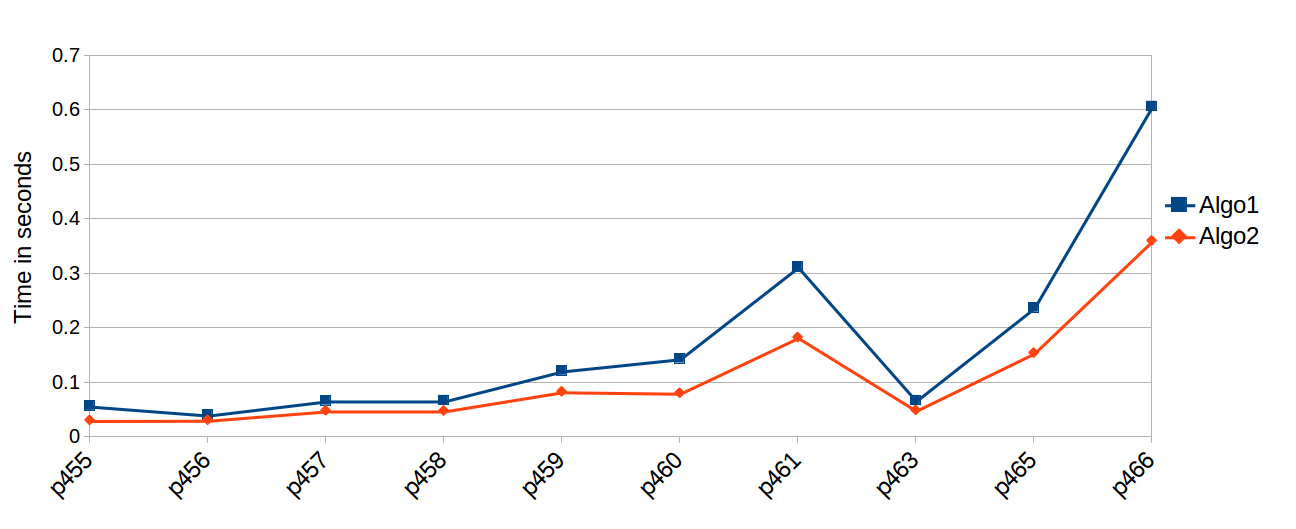
\includegraphics[scale = 0.45]{es3.png}
  \caption{Running Time comparison for Both Algorithms $algo1$ and $algo2$ on P4E dataset}
\end{figure}

\textbf{2. BCD Dataset :-} B, C, D are the instances of random generated graph with edges weights between 1 and 10. Out of these instances, we run both the algorithms on some of the instances of these dataset, as tabulated~\cite{koch}.\\ 


 \begin{figure}[H]
      \centering
    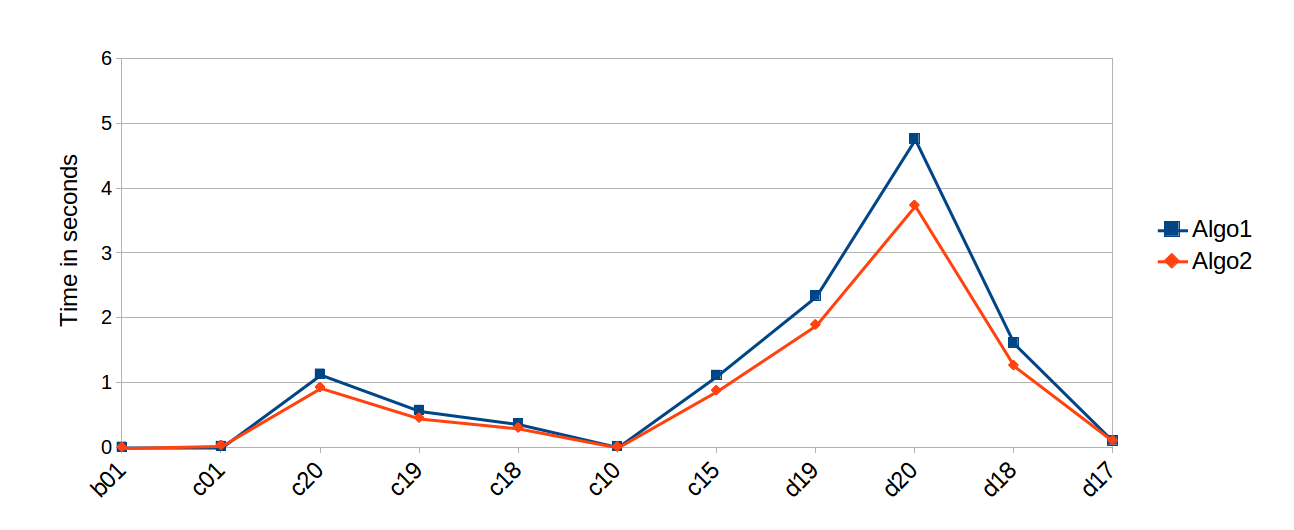
\includegraphics[scale = 0.45]{es2.png}
  \caption{Running Time Comparison for Both Algorithms $algo1$ and $algo2$ on B, C, D dataset}
\end{figure}


\begin{table}[H]
% \caption{My caption}
\label{my-label}
\begin{center}
\begin{tabular}{|l|l|l|l|l|l|}
\hline
Name & $|V|$      & $|E|$      & $|S|$      & DC         & Opt       \\ \hline
b01    &  50       &  63      &    9   &  Ls         &  82  \\ \hline
c01    &  500       &  625      &    10   &  Ps         &  144  \\ \hline
c10    &  500       &  1000      &    250   &  Ps         &  1093  \\ \hline
c15    &  500       &  2500      &    250   &  Ls         &  556  \\ \hline
c18    &  500       &  12500      &    250   &  Ps         &  113  \\ \hline
c19    &  500       &  12500      &    250   &  Ps         &  146  \\ \hline
c20    &  500       &  12500      &    250   &  Ls         &  267  \\ \hline

d17    &  1000       &  25000      &    10   &  Pm       &  23  \\ \hline
d18    &  1000       &  25000      &    167   &  Ps       &  223  \\ \hline

d19    &  1000       &  25000      &    250   &  Ps       &  310  \\ \hline
d20    &  1000       &  25000      &    500   &  Ls      &   537  \\ \hline
% P455    &  100       &  4950      &    5   &  Ps       &  1138  \\ \hline
\end{tabular}
\end{center}
\caption{B, C, D are the instances}
\end{table}

As we can see in all the cases, for all the instances B, C, D our algorithm $algo2$ taking less running time than the algorithm $algo2$.


\textbf{3. E Dataset :-} These instances are for the sparse graph that generated randomly with edges weights in between 1 to 10. DC means difficulty level of the problem.

Running times are change according to the change eigher in the number of edges or number of terminals present in the graphs. As we can see running times in figure 4.3 and figure 4.4, for the instances of table 4.1 and 4.2.  
 
\begin{table}[H]
% \caption{My caption}
\label{my-label}
\begin{center}
\begin{tabular}{|l|l|l|l|l|l|}
\hline
Name & $|V|$      & $|E|$      & $|S|$      & DC         & Opt       \\ \hline

 e01.stp &  2500      &  3125      &   5    & Ps   & 111    \\ \hline
 e02.stp &  2500      &  3125      &  10    & Ps   & 214     \\ \hline
 e03.stp &  2500      &  3125      &  417   & Ps   & 4013    \\ \hline
 e04.stp &  2500      &  3125      &  625   & PS   & 5101    \\ \hline
 e05.stp &  2500      &  3125      &  1250  & Ps   & 8128     \\ \hline
 e06.stp &  2500      &  5000      &  5     & Ps   & 73     \\ \hline
 e07.stp &  2500      &  5000      &  10    & Pm   & 145      \\ \hline
 e08.stp &  2500      &  5000      &  417   & Pm   & 2640       \\ \hline
 e09.stp &  2500      &  5000      &  625   & Pm   & 3604            \\ \hline
 e10.stp &  2500      &  5000      &  1250  & Pm   & 5600      \\ \hline
 e11.stp &  2500      &  12500     &  5     & Pm   & 34         \\ \hline
 e12.stp &  2500      &  12500     &  10    & Pm   & 67        \\ \hline
 e13.stp &  2500      &  12500     &  417   & Pm   & 1280          \\ \hline
 e14.stp &  2500      &  12500     &  625   & Pm   & 1732            \\ \hline
 e15.stp &  2500      &  12500     &  1250  & Ps   & 2784        \\ \hline
 e16.stp &  2500      &  62500     &  5     & Ph   & 15       \\ \hline
 e17.stp &  2500      &  62500     &  10    & Ph   & 25       \\ \hline
 e18.stp &  2500      &  62500     &  417   & NPh  & 564       \\ \hline
 e19.stp &  2500      &  62500     &  625   & Pm   & 758    \\ \hline
 e20.stp &  2500      &  62500     &  1250  & Ls   & 1342     \\ \hline
 
% P455    &  100       &  4950      &    5   &  Ps       &  1138  \\ \hline
\end{tabular}
\end{center}
\caption{E instances}
\end{table}


 \begin{figure}[H]
      \centering
    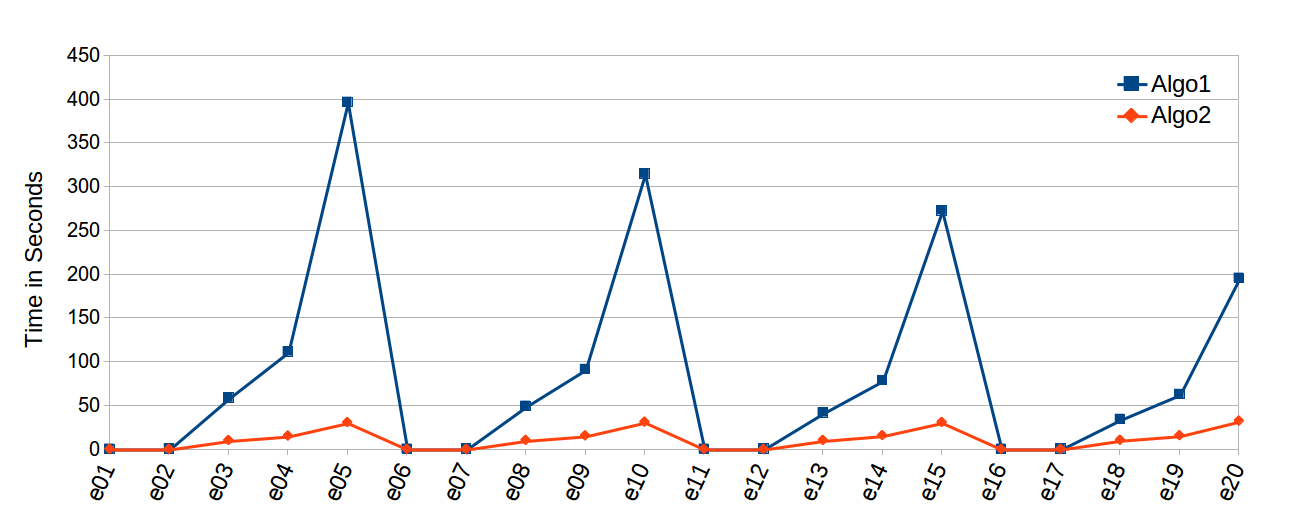
\includegraphics[scale = 0.45]{anilfinal.png}
  \caption{Running Time Comparison for Both Algorithms $algo1$ and $algo2$ on E dataset}
\end{figure}


\section{Computational Results}
Computational experiments were performed on test data set with quite different characteristics. All instance are available from the repository steinlib ~\cite{koch}. We run both the algorithms $algo1$ and $algo2$ on these instance. The running times for both the algorithms are present in the table 4.1, and table 4.2. First heuristic algorithm $algo1$ given by L. Kou, G. Markowsky, and L. Berman ~\cite{markowsky}. Second algorithm $algo2$ propose in this thesis. Both algorithms were run on the same dataset, and we calculate their running time, how much time both algorithm are taking, in almost all cases our propose algorithm is taking less time as compare to the previous heuristic algorithm. Representations in tables are as follows, $|V|$ number of vertices present in the graph, $|E|$ number of edges present in the graph, $|S|$ number of terminals present in the graph. Running time is in seconds present for both the algorithms. 

All the results in tables 4.3, 4.4, 4.5 obtained for both the programs by running these programs using G++ compiler on a machine with configuration as Intel(R) core(TM) i5-2320 CPU @ 3.00Hz 3.00 GHz processor, with RAM 4.00GM and system type 32-bit operating system. This time may change according to the machine configurations.
    

\begin{table}[H]
% \caption{My caption}
\label{my-label}
\begin{center}
\begin{tabular}{|l|l|l|l|l|l|l|l|l|}
\hline
Instance & \multicolumn{4}{l|}{Heuristic Algo1} & \multicolumn{4}{l|}{Heuristic Algo2} \\ \hline
         & $|V|$      & $|E|$      & $|S|$      & Time in Sec     & $|V|$      & $|E|$      & $|S|$     & Time in Sec    \\ \hline
     b01.stp    &  50       &    63      &     9   &  0.00369       &  50       &    63      &     9    & 0.000967        \\ \hline
     c01.stp    &  500      &    625     &     5   &  0.016047      &  500      &    625     &     5    &  0.034286    \\ \hline
     c20.stp    &  500      &   12500    &     250   &  1.13426     &  500      &   12500    &     250  &  0.928982 \\ \hline

     c19.stp    &  500      &   12500    &     150   &  0.573434      &  500       &   12500    &     150   &  0.456435 \\ \hline
     c18.stp    &  500      &   12500    &     83    &  0.369872       &  500      &   12500    &     83    &  0.30325 \\ \hline

     c16.stp    &  500      &   12500    &     5   &  0.015228      &  500      &   12500    &     5    &  0.010057 \\ \hline

     c15.stp    &  500      &   12500    &     250   &  1.11433      &  500      &   12500    &     250   &  0.879228 \\ \hline
    
     % es10fst.stp     &  18   v   &   20     &     10    &  0.021338      &  18       &   20     &     10    &  0.0582559   \\ \hline
     % att48fst.stp    &  139      &   202    &     48    &  0.123454      &  139      &   202    &     48    &  0.156677  \\ \hline
     % pr136fst.stp    &  196      &   250    &     136   &  0.408418      &  196      &   250    &     136   &  0.452413 \\ \hline
     d19.stp    &  1000      &   25000    &     250   &  2.34159      &  1000      &   25000    &     250   &  1.8951 \\ \hline
     d20.stp    &  1000      &   25000    &     500   &  4.76639      &  1000      &   25000    &     500   &  3.74008 \\ \hline
     d18.stp    &  1000      &   25000    &     167   &  1.61377      &  1000      &   25000     &     167   &  1.26696 \\ \hline
     d17.stp    &  1000      &   25000    &     10    &  0.10314       &  1000      &   25000    &      10   &  0.105337 \\ \hline
     
     % rd400fst.stp &  1001       &   1419       &   400    &  1.43076      &  1001       &   1419       &   400    &  1.50568 \\ \hline
     u574fst.stp &  990       &   1258       &   574    &  5.17052      &  990       &   1258       &   574    &  2.18517 \\ \hline
     p455.stp &  100       &   4950       &   5    &    0.0573699      &  100       &   4950       &   5    &    0.0309451 \\ \hline
     p456.stp &  100       &   4950       &   5    &    0.040837      &  100       &   4950       &   5    &    0.031431 \\ \hline
     p457.stp &  100       &   4950       &   10    &    0.0669429      &  100       &   4950       &   10    &    0.0486231 \\ \hline
     p458.stp &  100       &   4950       &   10    &    0.067569      &  100       &   4950       &   10    &    0.0483148 \\ \hline
     p459.stp &  100       &   4950       &   10    &    0.121697      &  100       &   4950       &   10    &    0.0835261 \\ \hline

     p460.stp &  100       &   4950       &   20    &    0.144033      &  100       &   4950       &   20    &    0.0809169 \\ \hline
     p461.stp &  100       &   4950       &   50   &    0.31225      &  100       &   4950       &   50    &    0.18301 \\ \hline
     p465.stp &  100       &   4950       &   40    &    0.237409      &  100       &   4950       &   40    &    0.154525 \\ \hline

     p466.stp &  200       &   19900       &   100    &    0.606883      &  200       &   19900       &   100    &    0.360251 \\ \hline

     

         % &        &        &        &           &        &        &       &          \\ \hline
         % &        &        &        &           &        &        &       &          \\ \hline
\end{tabular}
\end{center}
\caption{Detail results of computation on test instance}
\end{table}




\begin{table}[ht]
% \caption{My caption}
\label{my-label}
\begin{center}
\begin{tabular}{|l|l|l|l|l|l|l|l|l|}
\hline
Instance & \multicolumn{4}{l|}{Heuristic Algo1} & \multicolumn{4}{l|}{Heuristic Algo2} \\ \hline
         & $|V|$      & $|E|$      & $|S|$      & Time in Sec     & $|V|$      & $|E|$      & $|S|$     & Time in Sec    \\ \hline
     % d17.stp    &  1000      &   25000    &     10    &  0.10314       &  1000      &   25000    &      10   &  0.105337 \\ \hline
     es10fst15.stp &  16       &   18       &     10    &  0.71318       &  16        &   18       &      10   &  0.04878 \\ \hline
     es10fst14.stp &  24       &   32       &     10    &  0.721951       &  24        &   32       &      10   &  0.04708 \\ \hline
     es10fst13.stp &  18       &   21       &     10    &  0.72192        &  18        &   21       &      10   &  0.046977 \\ \hline

     % berlin52fst.stp & 89      &   104      &     52    &  0.318259        &  89        &   104      &    52   &  0.185827 \\ \hline
     es10fst13.stp &  18       &   21       &     10    &  0.72192        &  18        &   21       &      10   &  0.046977 \\ \hline
     es10fst13.stp &  18       &   21       &     10    &  0.72192        &  18        &   21       &      10   &  0.046977 \\ \hline
     es10fst13.stp &  18       &   21       &     10    &  0.72192        &  18        &   21       &      10   &  0.046977 \\ \hline
     es10fst13.stp &  18       &   21       &     10    &  0.72192        &  18        &   21       &      10   &  0.046977 \\ \hline
    
     % p466.stp &  200       &   19900       &   100    &    0.606883      &  200       &   19900       &   100    &    0.360251 \\ \hline

     es20fst101.stp  & 29  &   28       &   20    &  0.123531     &  29       &   28       &   20    &    0.08129 \\ \hline
     es20fst102.stp  & 29  &   28       &   20    &  0.125359     &  29       &   28       &   20    &    0.0812831 \\ \hline
     es20fst103.stp  & 27  &   26       &   20    &  0.132646     &  27       &   26       &   20    &    0.078793 \\ \hline
     es20fst104.stp  & 57  &   83       &   20    &  0.134467     &  57       &   83       &   20    &    0.0795579 \\ \hline
     es20fst105.stp  & 54  &   77       &   20    &  0.132566     &  54       &   77       &   20    &    0.0807161 \\ \hline
     es20fst106.stp  & 29  &   28       &   20    &  0.133814     &  29       &   28       &   20    &    0.0790079 \\ \hline
     es20fst111.stp  & 33  &   36       &   20    &  0.134738     &  33       &   36       &   20    &    0.0798302 \\ \hline
     es20fst113.stp  & 35  &   40       &   20    &  0.133753     &  35       &   40       &   20    &    0.0802221 \\ \hline
     es250fst01.stp  & 623  &   876       &  250    & 11.5419     & 623       &   876      &  250    &    0.893757 \\ \hline
     es250fst02.stp  & 542  &   719       &  250    & 11.5419     & 542       &   719      &  250    &    0.885769 \\ \hline

     es250fst03.stp  & 543  &   727       &  250    & 13.9157     & 543       &   727      &  250    &    0.890725 \\ \hline
     es250fst04.stp  & 604  &   842       &  250    & 11.2278     & 604       &   842      &  250    &    0.893235 \\ \hline
     es250fst05.stp  & 596  &   832       &  250    & 11.5419     & 596       &   832      &  250    &    0.891753 \\ \hline
     es250fst10.stp  & 662  &   951       &  250    & 10.8352     & 662       &   951      &  250    &    0.895662 \\ \hline
     es250fst11.stp  & 661  &   952       &  250    & 13.2844     & 661       &   952      &  250    &    0.900668 \\ \hline
     es250fst15.stp  & 713  &   1053       &  250    & 11.6048     &713       &   1053      &  250    &   0.90136 \\ \hline


         % &        &        &        &           &        &        &       &          \\ \hline
         % &        &        &        &           &        &        &       &          \\ \hline
\end{tabular}
\end{center}
\caption{Detail results of computation on test instance ES 10,20,250 fst}
\end{table}


\begin{table}[ht]
% \caption{My caption}
\label{my-label}
\begin{center}
\begin{tabular}{|l|l|l|l|l|l|l|l|l|}
\hline
Instance & \multicolumn{4}{l|}{Heuristic Algo1} & \multicolumn{4}{l|}{Heuristic Algo2} \\ \hline
         & $|V|$      & $|E|$      & $|S|$      & Time in Sec     & $|V|$      & $|E|$      & $|S|$     & Time in Sec     \\ \hline
 e01.stp &  2500      &  3125      &   5        &  0.361644       &  2500      &  3125      &   5       &  0.206146       \\ \hline
 e02.stp &  2500      &  3125      &  10        &  0.643139       &  2500      &  3125      &  10       &  0.327235       \\ \hline
 e03.stp &  2500      &  3125      &  417       &  58.8115        &  2500      &  3125      &  417      &  10.3275        \\ \hline
 e04.stp &  2500      &  3125      &  625       &  111.695        &  2500      &  3125      &  625      &  15.4805        \\ \hline
 e05.stp &  2500      &  3125      &  1250      &  396.873        &  2500      &  3125      &  1250     &  30.8221        \\ \hline
 e06.stp &  2500      &  5000      &  5         &  0.356108       &  2500      &  3125      &  5        &  0.205941       \\ \hline
 e07.stp &  2500      &  5000      &  10        &  0.628921       &  2500      &  5000      &  10       &  0.330493       \\ \hline
 e08.stp &  2500      &  5000      &  417       &  49.4262        &  2500      &  5000      &  417      &  10.4627        \\ \hline
 e09.stp &  2500      &  5000      &  625       &  91.5182        &  2500      &  5000      &  625      &  15.6537        \\ \hline
 e10.stp &  2500      &  5000      &  1250      &  314.90         &  2500      &  5000b     &  1250     &  31.3128        \\ \hline
 e11.stp &  2500      &  12500     &  5         &  0.349082       &  2500      &  12500     &  5        &  0.202747       \\ \hline
 e12.stp &  2500      &  12500     &  10        &  0.607044       &  2500      &  12500     &  10       &  0.32562        \\ \hline
 e13.stp &  2500      &  12500     &  417       &  41.892         &  2500      &  12500     &  417      &  10.4017        \\ \hline
 e14.stp &  2500      &  12500     &  625       &  78.7861        &  2500      &  12500     &  625      &  15.9379        \\ \hline
 e15.stp &  2500      &  12500     &  1250      &  272.956        &  2500      &  12500     &  1250     &  30.9364        \\ \hline
 e16.stp &  2500      &  62500     &  5         &  0.337468       &  2500      &  62500     &  5        &  0.205354       \\ \hline
 e17.stp &  2500      &  62500     &  10        &  0.595741       &  2500      &  62500     &  10       &  0.331765       \\ \hline
 e18.stp &  2500      &  62500     &  417       &  34.4145        &  2500      &  62500     &  417      &  10.6498        \\ \hline
 e19.stp &  2500      &  62500     &  625       &  62.9514        &  2500      &  62500     &  625      &  15.8446        \\ \hline
 e20.stp &  2500      &  62500     &  1250      &  195.743        &  2500      &  62500     &  1250     &  32.5236        \\ \hline
 
\end{tabular}
\end{center}
\caption{Detail results of computation on test instance E}
\end{table}

% \section{Conclusion} All the results in tables 4.3, 4.4, 4.5 obtained for both the programs by running these programs using G++ compiler on a machine with configuration as Intel(R) core(TM) i5-2320 CPU @ 3.00Hz 3.00 GHz processor, with RAM 4.00GM and system type 32-bit operating system. This time may change according to the machine configurations.


